% GB4 -- DD2 Project 1, Option 2: Finding Cells Worth Adding -- technical report.
% Build from this folder:  pdflatex report.tex  (run twice)  ->  report.pdf
% Figures are read from ../results/ (the files the flow wrote); every number below
% comes from a file under results/ or libs/cellweaver/ named next to it.
\documentclass[10pt,a4paper]{article}
\usepackage[margin=2cm]{geometry}
\usepackage[T1]{fontenc}
\usepackage{lmodern}
\usepackage{microtype}
\usepackage{booktabs}
\usepackage{tabularx}
\usepackage{graphicx}
\usepackage{amsmath}
\usepackage{xcolor}
\usepackage{enumitem}
\usepackage{caption}
\usepackage[hidelinks]{hyperref}
\graphicspath{{../results/}}
\setlist{nosep,leftmargin=*}
\captionsetup{font=small,labelfont=bf}
\makeatletter
\setlength{\@fptop}{0pt}
\setlength{\@fpsep}{12pt}
\setlength{\@fpbot}{0pt plus 1fil}
\makeatother
\newcommand{\um}{\ensuremath{\mu\mathrm{m}^2}}
\newcommand{\file}[1]{\texttt{\detokenize{#1}}}
\newcommand{\cell}[1]{\texttt{\detokenize{#1}}}
\newcommand{\fillin}[1]{\textcolor{red}{[#1]}}

\begin{document}

%======================================================================
\begin{titlepage}
\centering
\vspace*{3cm}
{\Large CSCE 3304 Digital Design II -- Fall 2026\par}
\vspace{0.6cm}
{\LARGE\bfseries DD2 Project 1, Option 2:\\[0.2cm] Finding Cells Worth Adding\par}
\vspace{0.4cm}
{\large Technical report\par}
\vspace{1.5cm}
{\large Group GB4 (cell names use the prefix \cell{dd2_g4__})\par}
\vspace{0.6cm}
\begin{tabular}{ll}
Omar Abdel Motalb & 900232118\\
Noor Elshahidi & 900230000\\
Mohamed Azouz & 900225230\\
\end{tabular}
\vspace{1.2cm}

\begin{tabular}{rl}
Option: & 2 (three-student group, cell finder; real cells from the provided generator)\\
Use of AI: & a development aid; the tool runs no model\\
Submitted: & Tuesday 10 November 2026\\
Tested commit: & \href{https://github.com/IOI-dot/dd2-cell-finder/commit/b8abd7d06e2ec9f195dcd4362c9d1835a5087284}{\texttt{b8abd7d06e2ec9f195dcd4362c9d1835a5087284}}\\
Submission tag: & \href{https://github.com/IOI-dot/dd2-cell-finder/tree/final}{\texttt{final}}\\
\end{tabular}
\end{titlepage}

%======================================================================
\section{Introduction}

The sky130\_fd\_sc\_hd (HD) library already offers most small single-stage CMOS functions.
The question of Option~2 is whether any small function that real designs compute again and
again is missing from HD, and whether adding a cell for it reduces the area Yosys and ABC reach.

We built a deterministic Python tool (\file{src/dd2} and \file{src/dd2m2}) that
(1)~extracts and-inverter graphs (AIGs) from the designs, (2)~enumerates and checks every
4-input cut, (3)~classifies the cut functions, (4)~costs each class as an explicit static-CMOS
realization, (5)~checks each one against every combinational cell of the full HD Liberty,
(6)~estimates its area with a model fitted to HD's x1 cells, (7)~ranks the candidates on the
cells of the current mapping, (8)~writes Appendix~A requests and an extended Liberty file,
(9)~maps and measures every design with and without the new cells, proving each mapping with
ABC \texttt{cec}, (10)~selects up to ten cells greedily by remapping, (11)~replaces the
estimated cells by the characterized cells returned by the provided generator
(CellWeaver \texttt{scl-gen 0.1.0}), and (12)~repeats the mapping with one cell 30\% smaller.

For the six required designs, the ten cells chosen with estimated
areas reduce the best-of-both area by 391.6~\um{} (0.457\%). With the real generator cells the
reduction is 148.9~\um{} (0.174\%), but \emph{no real cell is instantiated in any of the 20
mappings}: every real cell is 2.2--8.8$\times$ larger than its estimate, and ABC found no place
where one was cheaper than the HD logic it would replace. The remaining real-cell saving comes from ABC's \texttt{\&nf} choosing a
different mapping of existing HD gates once the library changes, and is of the same order as the
change the 30\% experiment produces on its own. We therefore conclude that
these cells, as generated, do not save area on these designs.

%======================================================================
\section{Method}
\label{sec:method}

Table~\ref{tab:steps} maps the twelve steps of the handout to commands and code.
\texttt{make all} runs M1, M2, a fresh best-of-all greedy search and the real-cell run;
\texttt{make reproduce} reruns the real-cell experiment from the published selection.

\begin{table}[h]
\centering\small
\caption{Steps of handout \S4, their commands and modules.}
\label{tab:steps}
\begin{tabularx}{\textwidth}{@{}l>{\raggedright\arraybackslash}p{4.3cm}X@{}}
\toprule
Step & Command & Code \\
\midrule
1 Extract AIG & \texttt{make m1-aigs} & \file{dd2/aig.py} \\
2 Enumerate cuts & \texttt{make m1-cuts} & \file{dd2/cuts.py}, independent check \file{dd2/cutcheck.py} \\
3 Classify & \texttt{make m1-cuts}, \texttt{make m1-hdclasses} & \file{dd2/boolfn.py}, \file{dd2/hdclasses.py} \\
4 Cost & \texttt{make m2-candidates} & \file{dd2m2/cost.py}, \file{dd2/stage.py} \\
5 Redundancy & \texttt{make m1-redundancy} (self-test) & \file{dd2/redundancy.py} \\
6 Area model & \texttt{make m2-fit} & \file{dd2m2/areamodel.py}, \file{dd2m2/cost.py} \\
7 Rank & \texttt{make m2-candidates} & \file{dd2m2/candidates.py}, \file{dd2m2/cones.py} \\
8 Requests, Liberty & \texttt{make m2-library} & \file{dd2m2/candidates.py}, \file{dd2m2/library.py}, \file{dd2/interface.py} \\
9 Map and measure & \texttt{make m1-baseline}, \texttt{make m2-map} & \file{dd2m2/evaluate.py}, \file{dd2m2/measure.py}, \file{dd2m2/tutorials.py} \\
10 Greedy selection & \texttt{make m3-estimated-best} & \file{dd2m2/final_flow.py} \\
11 Real cells & \texttt{make m3-real} / \texttt{make reproduce} & \file{dd2m2/generator.py}, \file{dd2m2/final_flow.py} \\
12 Sensitivity & part of steps 10 and 11 & \file{dd2m2/generator.py} (\texttt{scale\_cell\_area}) \\
Demo & \texttt{make demo IN=<design.v>} & \file{dd2m2/final_flow.py} (\texttt{demo}) \\
\bottomrule
\end{tabularx}
\end{table}

\paragraph{Step 1: AIGs.} Each design is read with Yosys, synthesized with
\texttt{synth -flatten -top}, its asynchronous flip-flops converted with \texttt{async2sync;
dffunmap}, then \texttt{aigmap; write\_aiger -zinit}. With Yosys~0.33 the AND counts equal
handout Table~2 for all six required designs, and the latch count of the plain AIG equals the
flip-flop count after \texttt{synth}. The restructured AIG is written by ABC with
\texttt{strash; dch -f; strash} (the last \texttt{strash} removes the choice nodes \texttt{dch}
leaves); it must have the same outputs, no choice nodes, and pass \texttt{cec} against the synth AIG.

\paragraph{Step 2: cuts.} Our enumerator (\file{dd2/cuts.py}) computes, for every AND node, the
merges of its fanins' cuts with at most $k=4$ leaves, drops dominated cuts, and carries a truth
table for each cut, input~0 being the least significant bit of the row index as in Appendix~A.
A separate checker (\file{dd2/cutcheck.py}), which shares no code with the enumerator, walks the
AIG from the root to the leaves for each of the $2^k$ leaf assignments and compares every bit.
Every cut of every AIG is checked, and the number checked must equal the number enumerated and
the number written.

\paragraph{Step 3: classes.} Each cut function is first reduced to its essential support (the leaves
it really depends on). Truth tables are canonicalized as the minimum table over three groups:
P (input permutations; this is ``up to input order'' of Table~4 and the key of our candidates),
PN (permutations and output inversion, the classes of the handout's step~3), and NPN (also input
inversions). PN is the count that matters for CMOS: an output inversion is absorbed by choosing
the complementary pull-up/pull-down pair, but every inverted input costs an inverter, i.e.\ two
transistors and an extra stage, so NPN classes merge functions with different costs.

\paragraph{Step 4: cost.} \file{dd2m2/cost.py} builds explicit static-CMOS realizations and keeps the one with
the fewest transistors (ties: fewer stages, then fewer inverters). It tries (a)~a NAND2/NAND3
network from an exact minimum-literal sum of products, (b)~the dual NOR2/NOR3 network from the
product of sums, and (c)~factored single stages $Y=\overline{F}$, with $F$ a series-parallel formula
of up to 6 literals (12 transistors) in which an input may repeat, under all input-inversion masks
and with or without an output inverter. Each literal costs one NMOS and one PMOS; AND is series in
the pull-down and parallel in the pull-up. New candidates are limited to 3 transistors in series per
stage; HD calibration cells may use 4 (NAND4/NOR4 exist natively). Every returned realization is
evaluated against the candidate's full truth table.

\paragraph{Step 5: redundancy.} \file{dd2/redundancy.py} compares a candidate, on its essential support,
with every single-output combinational cell of the full HD Liberty (all drives and kinds), using
each cell's \texttt{function} attribute. The tests are applied in the order of Table~3 and the first
match wins: \emph{Exists} (same P-class), \emph{Exists with an inverter} (equal after inverting the
output or exactly one input), \emph{Contained} (equal to an HD cell with each HD input tied to a
candidate input or to 0/1, by exhaustive enumeration of the ties), else \emph{New}. The decision rule
is the handout's: Exists is dropped; Exists-with-an-inverter is kept only if its estimated area is
smaller than the matched cell plus the smallest HD inverter; Contained is kept only if its estimated
area is smaller than the matched cell; New is kept.

\paragraph{Step 6: area model.} Width in 0.46~$\mu$m sites is modelled as
$w = c_0 + c_1 T + c_2 (S-1) + c_3 I$ ($T$ transistors, $S$ stages, $I$ inverters of the step~4
realization), fitted by non-negative least squares to the x1 cells of the reduced library with at
most 4 inputs, and rounded up to a whole site; area $= w\times 2.72\times 0.46 = w\times 1.2512$~\um.

\paragraph{Step 7: ranking.} Frequency in the AIG is a poor proxy, so the ranking is tied to the cells of
the current mapping (\file{dd2m2/cones.py}). For every baseline netlist (both scripts) we enumerate cuts
of up to 4 leaves over mapped cells, compute the cut's function from the cells' Liberty functions, and
count as reclaimable only the cells inside the cone with no consumer outside it. For each candidate,
design and script we greedily accept non-overlapping occurrences whose reclaimable area exceeds the
candidate's estimated area, and predict the resulting best-of-both saving over the six required
designs. Eligible candidates are sorted by that prediction. The prediction ignores overlap between
different candidates and ABC's own choices; it only orders the greedy search.

\paragraph{Step 8: requests and Liberty.} Each request follows Appendix~A: name
\cell{dd2_g4__n<k>_<tt>_1}, inputs \texttt{A..D}, output \texttt{Y}, the realization's expression, the
truth table in hexadecimal, sizing \texttt{hd} and the estimated area; it is validated (expression
and truth table must agree) before use. The Liberty writer appends one cell per request inside the
library group of \file{hd_reduced.lib}: the estimated area, input capacitance 0.0024~pF, the output
function, and one timing arc per input whose \texttt{timing\_sense} is derived from the truth table,
with scalar placeholder delays of 0.10~ns. The written file is parsed back and each cell's function
must reproduce its truth table; Yosys \texttt{read\_liberty -lib} must report $189+N$ cells
(``Imported 199 cell types'' in every \file{liberty_import.log} of M2 and M3).

\paragraph{Step 9: mapping and checks.} Mapping uses the commands of \file{given/scripts/map.sh}
verbatim, with scripts A (\texttt{+strash;dch,-f;amap;topo}) and B
(\texttt{+strash;\&get,-n;\&dch,-f;\&nf,-R,1000;\&put}); we only add \texttt{write\_rtlil} of the
synthesized design before \texttt{dfflibmap} (the ``gold'') and \texttt{stat -json}. Each mapping is
then proved: gold and the Liberty-expanded mapped netlist are both converted with
\texttt{async2sync; dffunmap; aigmap}, register outputs are given names traced back to the RTL
instances, the two AIGs are aligned by a bijective name match (never by latch order), and ABC
\texttt{cec} must report ``Networks are equivalent''. A Yosys \texttt{equiv\_induct} run is kept only
as a bounded diagnostic. For SPM and the multiplier, the original Tutorial~4 and Tutorial~2 testbenches
run on the RTL and on all four gate-level netlists with Icarus, using cell models written from the
same Liberty (functional, zero-delay). OpenSTA reports the worst arrival time under fixed comparison
constraints: a 100~ns clock on the clock port (or a virtual clock), 0.1~ns input and clock slew,
0.01~pF output load, zero input/output delay.

\paragraph{Step 10: greedy selection.} \file{final_flow.py} implements the handout's rule in two
variants. \texttt{make m3-estimated} takes the first ranked candidate that lowers the total.
The published run, \texttt{make m3-estimated-best}, is stricter: in each round it remaps the six
required designs with both scripts for \emph{every} remaining eligible candidate added to the current
set, keeps the candidate with the lowest total best-of-both area if that total drops, and stops after
10 cells or when no candidate helps. It ran 7{,}735 trial libraries (778 in round~1 down to 769 in
round~10; \file{results/m3/estimated-best/selection_trials.csv}). The chosen set is then mapped
again with full checks; the verified total must equal the trial total.

\paragraph{Step 11: real cells.} \file{generator.py} accepts a response only if its status is
\texttt{pass}, its six checks are exactly DRC~0, LVS and RC-LVS \texttt{match}, truth table
\texttt{pass}, abutment~0 and layers \texttt{pass}; its Liberty holds exactly one cell with the
requested name and pins, whose function equals the requested truth table and whose area equals the
response; and it carries non-scalar \texttt{cell\_rise}, \texttt{cell\_fall},
\texttt{rise\_transition} and \texttt{fall\_transition} tables. The real-run baseline must be identical
(areas, input hashes, Yosys version) to the estimated-run baseline. The cell-by-cell curve remaps
every prefix of the chosen order.

\paragraph{Step 12: sensitivity.} The first chosen cell's \texttt{area} is multiplied by 0.7 in the
Liberty and every design is mapped and verified again.

The selection objective is the sum over the six required designs of the smaller of
the A and B areas, the number the conclusion rests on. SPM and the multiplier (tutorial
designs) and pic16 and p16c5x (same instruction set as risc8) are measured with every library but are
not part of the objective, so they act as held-out designs.

%======================================================================
\section{Verification}
\label{sec:verif}

\texttt{make test} first verifies the SHA-256 checksums of the frozen broken cases, then runs the
pytest suite; the last recorded run passed 101 tests (\file{results/validation/tests.log}).
Table~\ref{tab:checks} lists each check and the deliberately broken case it must reject.

\begin{table}[h]
\centering\small
\caption{Checks and their broken cases (all run by \texttt{make test}).}
\label{tab:checks}
\begin{tabularx}{\textwidth}{@{}>{\raggedright\arraybackslash}p{3.6cm}X@{}}
\toprule
Check & Broken case that must fail \\
\midrule
Cut truth tables (\file{cutcheck.py}) & \file{tests/broken/wrong_truth_table.{aig,json}}: a real 4-leaf cut of cpu8 whose
truth table \texttt{0x1555} has bit 5 flipped to \texttt{0x1575}; the check and \texttt{dd2 cutcheck} reject it, and an empty cut file also fails. \\
Redundancy (\file{redundancy.py}) & \file{tests/broken/hd_cell_as_candidate.json}: HD's \cell{a21oi} function written as
\texttt{!(P | (Q \& R))} with renamed, reordered inputs must be \emph{Exists}. The self-test also requires all 323 HD cells to be Exists. \\
Liberty accepted by Yosys & \file{tests/broken_proposed/yosys_rejects.lib} (a missing \texttt{;}): Yosys \texttt{read\_liberty} must exit non-zero.
\file{tests/broken/invalid_function.lib} (a \texttt{\$} operator) must be rejected by our own Liberty reader. \\
Mapping equivalence (ABC \texttt{cec}) & \file{tests/m2/test_equivalence.py} maps an AND gate, then replaces the mapped netlist by an OR:
\texttt{cec} must fail. \file{tests/broken_proposed/nonequivalent_restructured.aig} (one fanin polarity of cpu8's last AND flipped) must fail \texttt{cec} against the cpu8 AIG. \\
Gate-level simulation & A wrong gate function must fail the original multiplier testbench; a run without the pass marker, with a non-zero exit code or an ERROR line fails. \\
OpenSTA & A tool error cannot be hidden by a numeric marker in the log. \\
Requests and responses & Contract tests reject requests whose expression and truth table disagree and responses that are not \texttt{pass}. \\
\bottomrule
\end{tabularx}
\end{table}

In the measured runs every
one of the 80 mappings of M3 (10 designs $\times$ 2 scripts $\times$ baseline/extended, for the
estimated and the real libraries) passed \texttt{cec}, every OpenSTA run passed, and SPM and the multiplier
passed their RTL and all four gate-level simulations (\file{results/m3/*/tutorial_simulations.json}).

%======================================================================
\section{Results}
\label{sec:results}

\subsection{Baseline: Table 1 reproduced}

With Yosys~0.33 all 24 areas of handout Table~1 match to the printed
0.1~\um{} (\file{results/m1/table1.csv}). The reduced library costs at most 0.49\% (arlet6502, A)
over the usable library. The M2 and M3 runs use Yosys~0.70+240, whose baseline areas differ
slightly (e.g.\ cpu8~A 4{,}165.2 instead of 4{,}186.5~\um); every comparison below uses baseline and
extended libraries mapped with the same tool in the same run.

\subsection{AIGs, cuts and classes}

\begin{table}[h]
\centering\small
\caption{AIG size, checked 4-input cuts and classes before (synth) and after ABC restructuring
(\file{results/m1/aigs/compare.csv}, \file{results/m1/cuts/summary.csv}). Classes are over each cut's essential
support; ``4-in'' counts classes of functions that depend on all four inputs.}
\label{tab:aig}
\begin{tabular}{@{}lrrrrrrrrrr@{}}
\toprule
& & \multicolumn{4}{c}{synth AIG} & \multicolumn{4}{c}{restructured AIG (\texttt{dch})} \\
\cmidrule(lr){3-6}\cmidrule(lr){7-10}
Design & FFs & ANDs & cuts & PN (4-in) & NPN (4-in) & ANDs & cuts & PN (4-in) & NPN (4-in) \\
\midrule
cpu8 & 82 & 1{,}265 & 10{,}725 & 195 (166) & 63 (50) & 1{,}108 & 9{,}003 & 200 (171) & 64 (54) \\
dsp8 & 72 & 1{,}973 & 16{,}445 & 200 (172) & 54 (43) & 1{,}534 & 13{,}004 & 205 (176) & 56 (45) \\
arlet6502 & 143 & 3{,}221 & 27{,}091 & 205 (177) & 51 (40) & 2{,}754 & 21{,}132 & 209 (181) & 61 (50) \\
uart\_apb & 330 & 4{,}673 & 39{,}290 & 203 (170) & 45 (34) & 2{,}986 & 18{,}059 & 135 (114) & 38 (30) \\
risc8 & 696 & 7{,}750 & 57{,}178 & 173 (145) & 45 (34) & 6{,}589 & 44{,}172 & 177 (150) & 46 (36) \\
fir10 & 176 & 8{,}795 & 92{,}196 & 176 (148) & 43 (32) & 6{,}937 & 75{,}435 & 170 (145) & 43 (34) \\
\midrule
all six & & & & 342 (306) & 86 (73) & & & 326 (293) & 93 (81) \\
\bottomrule
\end{tabular}
\end{table}

Flip-flop and synth AND counts equal handout Table~2 for all six designs. Restructuring removes
12--36\% of the AND nodes and 16--54\% of the cuts (most on uart\_apb), and all 6 restructured AIGs pass \texttt{cec}
against their synth AIG with 12 total checks. All 423{,}730 cuts pass the exhaustive check with zero failures.
Across the six designs we find 306 four-input PN classes in the synth AIGs and 293 after
restructuring, against only 73 and 81 NPN classes: ignoring input inverters would merge roughly
four CMOS-distinct functions into each class, which is why PN is the count that matters.

\textbf{Class table of HD.} The full HD Liberty has 323 single-output combinational cells (105
excluded: 69 sequential, 13 tri-state, 12 without outputs, 10 with two outputs, 1 without inputs).
They fall into 40 PN classes, 19 NPN classes and 77 P-classes (\file{results/m1/hd_classes.csv},
\file{results/m1/hd_pn_classes.csv}). Only 12 PN classes of 4-input functions exist in HD
(e.g.\ \texttt{nor4}, \texttt{a211oi}, \texttt{a31oi}, \texttt{o22ai}, \texttt{a22oi}, \texttt{o211ai},
\texttt{nand4}, \texttt{and4bb}/\texttt{nor4bb}, \texttt{a2bb2oi}), against about 300 in the designs.

\subsection{Redundancy checker self-test (Table 4)}

\begin{table}[h]
\centering\small
\caption{Self-test against handout Table~4 (\file{results/m1/redundancy/self_test.json}). 3{,}904 P-classes depend on all four inputs.}
\label{tab:t4}
\begin{tabular}{@{}lrrl@{}}
\toprule
Group & Handout & Ours & Status \\
\midrule
Exists & 24 & 24 & match \\
Exists with an inverter & 20 & 20 & match \\
Contained & 38 & 38 & match \\
New & 3{,}822 & 3{,}822 & match \\
New, one static CMOS stage & 9 & 9 & match \\
New, one stage, $\le$3 in series, $\le$12 transistors & 5 & 6 & recorded difference \\
One stage, every input once & 8 (6 Exist, 2 Contained) & 8 (6 Exist, 2 Contained) & match \\
\bottomrule
\end{tabular}
\end{table}

All 323 HD cells classify as Exists, and six of seven rows match. For the row ``one stage, at most 3 in
series, at most 12 transistors'' we find six classes where the handout gives five. Each of the six has a
verified 12-transistor series-parallel form within the series limit
(\file{TA_M2/table4_witnesses.csv}): \texttt{0x0017}, \texttt{0x011F}, \texttt{0x013F}, \texttt{0x037F},
\texttt{0x077F} (the handout's \texttt{!((C\&D)|(A\&B\&(C|D)))}) and \texttt{0x17FF}
(\texttt{!(D\&((A\&B)|(C\&(A|B))))}). We did not tune the definition to reach five; the six witnesses,
the reference value and the original self-test are kept unchanged. The TA accepted
this result as submitted at checkpoint~2.

\subsection{Area model}

\begin{figure}
    \centering
    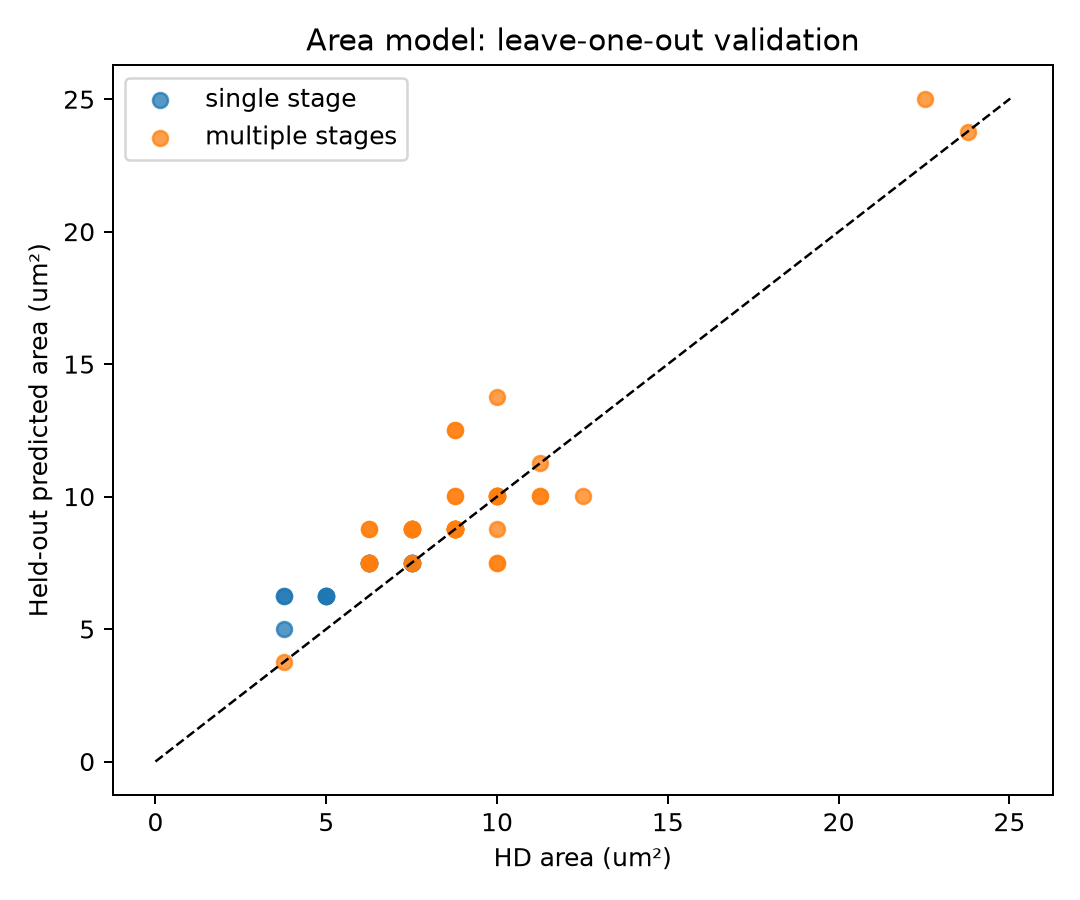
\includegraphics[width=0.8\linewidth]{m2/area_model_validation.png}
    \caption{Area model against HD x1 cells}
    \label{fig:area-model}
\end{figure}

The fit uses 61 HD x1 cells with at most four inputs (15 single-stage and 45 multi-stage realizations,
plus \cell{buf_1}, whose realization is a wire); 22 cells with five or six inputs are outside the
candidate domain and excluded (\file{results/m2/area_model_excluded.csv}). The coefficients are
$c_0=2.934$, $c_1=0.318$ sites per transistor, $c_2=0.496$ per extra stage and $c_3=0.083$ per inverter
(\file{results/m2/area_model.json}). Leave-one-out errors (each cell predicted by a model fitted without it):
mean absolute 14.6\%, median 14.3\%, maximum 66.7\%; in-sample, 25 of the 61 cells are predicted exactly.
The error is larger on single-stage cells (mean 23.1\%) than on multi-stage cells (11.8\%). The worst cases
are \cell{nand2_1} and \cell{nor2_1}, predicted at 5 sites instead of 3, and \cell{xor2_1}/\cell{xnor2_1},
predicted at 10 instead of 7, because our XOR realization (16 transistors, 3 stages) is costlier than HD's
custom 7-site layout.

\subsection{Candidates, ranking and the final set}

The candidate pool is every 2- to 4-input P-class seen in the AIG cuts or in the mapped cones of
the eight designs mapped in M2 (six required, SPM, multiplier): 833 functions
(\file{results/m2/ranked_candidates.csv}, \file{redundancy_report.csv}). The redundancy check removed
53 Exists (all 2-input functions, 21 three-input and 24 four-input classes) and 2 of the 28
Exists-with-an-inverter classes, whose estimate was not below the HD cell plus an inverter.
It kept 26 Exists-with-an-inverter, all 38 Contained and all 714 New classes: 778 eligible candidates.
Examples: \texttt{3:0x8E} is \cell{maj3_1} with input C inverted (estimate 11.26 vs.\ 10.01+3.75~\um, kept);
\texttt{3:0x2B} is Contained in \cell{mux4_2} with ties $A_0{=}1$, $A_1{=}A_2{=}A$, $A_3{=}0$ (10.01 vs.\
22.52~\um, kept); \texttt{4:0x07FF} $=\overline{D(C+AB)}$ is Contained in \cell{a32oi_1} with
$A_3{=}B_2{=}D$ (7.51 vs.\ 8.76~\um, kept).

The ten top-ranked candidates (the M2 set, \file{results/m2/selection.json}) were mapped together at
checkpoint~2 and \emph{increased} the six-design best-of-both total by 0.020\% (risc8 $-0.062$\%; all
others 0\%; \file{results/m2/summary.md}). The ranking predicted 1{,}778~\um{} for the first candidate
alone, which in fact added 1.25~\um{} (\S\ref{sec:freq}). This is why the final set is chosen by remapping.

\begin{table}[h]
\centering\small
\caption{Final set in greedy order (\file{results/m3/estimated-best/requests.json},
\file{results/m3/real/generator_cells.json}, \file{libs/cellweaver/responses.json}). T/S: transistors and stages
of our realization and of the generated cell; est./real: area in \um. Rank is the step~7 rank.}
\label{tab:final}
\setlength{\tabcolsep}{4pt}
\begin{tabular}{@{}rllllrrrrrr@{}}
\toprule
\# & Cell & Function (A = LSB) & Class & Rank & est.\ T/S & est. & real T/S & sites & real & ratio \\
\midrule
1 & \cell{n4_1bff} & \texttt{!D|(!A\&!B)|(A\&!C)} & New & 189 & 20/3 & 13.76 & 12/2 & 60 & 75.07 & 5.5 \\
2 & \cell{n4_00ae} & \texttt{!(D|(!A\&(!B|C)))} & New & 72 & 12/2 & 10.01 & 12/2 & 32 & 40.04 & 4.0 \\
3 & \cell{n4_07ff} & \texttt{!(D\&(C|(A\&B)))} & Contained & 28 & 8/1 & 7.51 & 8/1 & 13 & 16.27 & 2.2 \\
4 & \cell{n4_ead5} & \texttt{(!A\&!D)|(B\&C)|(A\&D)} & New & 33 & 22/3 & 15.01 & 20/2 & 100 & 125.12 & 8.3 \\
5 & \cell{n4_008a} & \texttt{!(!A|D|(!B\&C))} & New & 56 & 12/2 & 10.01 & 12/2 & 26 & 32.53 & 3.3 \\
6 & \cell{n4_8aa0} & \texttt{A\&(B|!C|!D)\&(C|D)} & New & 525 & 22/3 & 15.01 & 20/2 & 100 & 125.12 & 8.3 \\
7 & \cell{n4_88f8} & \texttt{(A\&B)|(C\&!D)} & Exists+inv & 36 & 12/3 & 10.01 & 14/2 & 70 & 87.58 & 8.8 \\
8 & \cell{n4_aaae} & \texttt{!(!A\&(!B|C|D))} & New & 77 & 12/2 & 10.01 & 12/2 & 23 & 28.78 & 2.9 \\
9 & \cell{n4_000e} & \texttt{!D\&!C\&(A|B)} & New & 88 & 10/2 & 8.76 & 12/2 & 26 & 32.53 & 3.7 \\
10 & \cell{n3_2e} & \texttt{(!B|!C)\&(A|B)} & Exists+inv & 131 & 16/3 & 12.51 & 12/2 & 24 & 30.03 & 2.4 \\
\bottomrule
\end{tabular}
\end{table}

Cell names in Table~\ref{tab:final} omit the prefix \cell{dd2_g4__} and the suffix \cell{_1}.
All ten responses have status \texttt{pass} with DRC~0, LVS and RC-LVS \texttt{match}.
The greedy search picked many low-ranked candidates (ranks 28--525): the ranking estimates savings
on the baseline mapping, while the greedy step measures what ABC does with the whole library.

\subsection{Table 5 with estimated and with real areas}

\begin{table}[p]
\centering\small
\caption{Table 5 with \textbf{estimated} areas (\file{results/m3/estimated-best/table5_estimated.csv}).
Reduction $=($baseline$-$extended$)/$baseline. Delay: OpenSTA worst arrival (ns), baseline $\to$ extended;
the new cells' timing is a 0.10~ns placeholder.}
\label{tab:t5est}
\begin{tabular}{@{}llrrrrlrr@{}}
\toprule
Design & Script & Baseline (\um) & With new cells (\um) & Reduction (\%) & New-cell inst. & Equivalence & \multicolumn{2}{c}{Delay (ns)} \\
\midrule
cpu8 & A & 4{,}165.2 & 4{,}165.2 & 0.00 & 0 & pass & 4.29 & 4.29 \\
 & B & 4{,}231.6 & 4{,}237.8 & $-$0.15 & 1 & pass & 5.28 & 4.50 \\
dsp8 & A & 5{,}811.8 & 5{,}798.1 & 0.24 & 5 & pass & 5.18 & 5.04 \\
 & B & 6{,}047.0 & 6{,}087.1 & $-$0.66 & 13 & pass & 6.06 & 5.77 \\
arlet6502 & A & 9{,}325.2 & 9{,}300.2 & 0.27 & 8 & pass & 6.56 & 6.45 \\
 & B & 9{,}527.9 & 9{,}495.4 & 0.34 & 23 & pass & 6.33 & 5.84 \\
uart\_apb & A & 12{,}773.5 & 12{,}751.0 & 0.18 & 7 & pass & 8.49 & 8.50 \\
 & B & 13{,}031.2 & 13{,}041.3 & $-$0.08 & 10 & pass & 4.28 & 4.28 \\
risc8 & A & 28{,}114.5 & 28{,}119.5 & $-$0.02 & 7 & pass & 24.42 & 24.31 \\
 & B & 28{,}094.4 & 27{,}893.0 & 0.72 & 12 & pass & 25.65 & 18.45 \\
fir10 & A & 25{,}463.2 & 25{,}334.3 & 0.51 & 36 & pass & 6.73 & 6.71 \\
 & B & 29{,}016.6 & 28{,}730.1 & 0.99 & 10 & pass & 7.64 & 8.42 \\
\midrule
spm & A & 2{,}869.0 & 2{,}869.0 & 0.00 & 0 & pass & 1.02 & 1.02 \\
 & B & 2{,}907.8 & 2{,}907.8 & 0.00 & 0 & pass & 0.69 & 0.69 \\
multiplier & A & 1{,}736.7 & 1{,}736.7 & 0.00 & 0 & pass & 4.37 & 4.37 \\
 & B & 1{,}954.4 & 1{,}945.6 & 0.45 & 3 & pass & 4.82 & 4.70 \\
pic16 & A & 30{,}336.6 & 30{,}301.6 & 0.12 & 12 & pass & 33.43 & 31.42 \\
 & B & 30{,}326.6 & 30{,}224.0 & 0.34 & 31 & pass & 27.11 & 24.52 \\
p16c5x & A & 29{,}548.3 & 29{,}487.0 & 0.21 & 12 & pass & 27.51 & 26.89 \\
 & B & 31{,}087.3 & 30{,}932.2 & 0.50 & 24 & pass & 27.51 & 21.69 \\
\bottomrule
\end{tabular}

\vspace{0.6cm}
\caption{Table 5 with \textbf{real} generator cells (\file{results/m3/real/table5_real.csv}). Delays use the
generator's characterized timing for the new cells and HD's for the rest.}
\label{tab:t5real}
\begin{tabular}{@{}llrrrrlrr@{}}
\toprule
Design & Script & Baseline (\um) & With new cells (\um) & Reduction (\%) & New-cell inst. & Equivalence & \multicolumn{2}{c}{Delay (ns)} \\
\midrule
cpu8 & A & 4{,}165.2 & 4{,}165.2 & 0.00 & 0 & pass & 4.29 & 4.29 \\
 & B & 4{,}231.6 & 4{,}239.1 & $-$0.18 & 0 & pass & 5.28 & 4.86 \\
dsp8 & A & 5{,}811.8 & 5{,}811.8 & 0.00 & 0 & pass & 5.18 & 5.18 \\
 & B & 6{,}047.0 & 6{,}054.6 & $-$0.12 & 0 & pass & 6.06 & 5.56 \\
arlet6502 & A & 9{,}325.2 & 9{,}325.2 & 0.00 & 0 & pass & 6.56 & 6.56 \\
 & B & 9{,}527.9 & 9{,}487.8 & 0.42 & 0 & pass & 6.33 & 6.07 \\
uart\_apb & A & 12{,}773.5 & 12{,}773.5 & 0.00 & 0 & pass & 8.49 & 8.49 \\
 & B & 13{,}031.2 & 13{,}023.7 & 0.06 & 0 & pass & 4.28 & 4.28 \\
risc8 & A & 28{,}114.5 & 28{,}114.5 & 0.00 & 0 & pass & 24.42 & 24.42 \\
 & B & 28{,}094.4 & 27{,}945.6 & 0.53 & 0 & pass & 25.65 & 18.37 \\
fir10 & A & 25{,}463.2 & 25{,}463.2 & 0.00 & 0 & pass & 6.73 & 6.73 \\
 & B & 29{,}016.6 & 28{,}757.6 & 0.89 & 0 & pass & 7.64 & 8.38 \\
\midrule
spm & A & 2{,}869.0 & 2{,}869.0 & 0.00 & 0 & pass & 1.02 & 1.02 \\
 & B & 2{,}907.8 & 2{,}907.8 & 0.00 & 0 & pass & 0.69 & 0.69 \\
multiplier & A & 1{,}736.7 & 1{,}736.7 & 0.00 & 0 & pass & 4.37 & 4.37 \\
 & B & 1{,}954.4 & 1{,}933.1 & 1.09 & 0 & pass & 4.82 & 4.82 \\
pic16 & A & 30{,}336.6 & 30{,}336.6 & 0.00 & 0 & pass & 33.43 & 33.43 \\
 & B & 30{,}326.6 & 30{,}226.5 & 0.33 & 0 & pass & 27.11 & 27.54 \\
p16c5x & A & 29{,}548.3 & 29{,}548.3 & 0.00 & 0 & pass & 27.51 & 27.51 \\
 & B & 31{,}087.3 & 30{,}972.2 & 0.37 & 0 & pass & 27.51 & 21.79 \\
\bottomrule
\end{tabular}
\end{table}

\begin{table}[h]
\centering\small
\caption{Best-of-both reductions: the smaller of the A and B areas on each side
(\file{best_of_both_estimated.csv}, \file{best_of_both_real.csv}). TOTAL is over the six required designs.}
\label{tab:best}
\begin{tabular}{@{}lrrrrrrr@{}}
\toprule
& Baseline & \multicolumn{3}{c}{Estimated cells} & \multicolumn{3}{c}{Real cells} \\
\cmidrule(lr){3-5}\cmidrule(lr){6-8}
Design & best (\um) & best (\um) & saving (\um) & red.\ (\%) & best (\um) & saving (\um) & red.\ (\%) \\
\midrule
cpu8 & 4{,}165.2 & 4{,}165.2 & 0.0 & 0.000 & 4{,}165.2 & 0.0 & 0.000 \\
dsp8 & 5{,}811.8 & 5{,}798.1 & 13.8 & 0.237 & 5{,}811.8 & 0.0 & 0.000 \\
arlet6502 & 9{,}325.2 & 9{,}300.2 & 25.0 & 0.268 & 9{,}325.2 & 0.0 & 0.000 \\
uart\_apb & 12{,}773.5 & 12{,}751.0 & 22.5 & 0.176 & 12{,}773.5 & 0.0 & 0.000 \\
risc8 & 28{,}094.4 & 27{,}893.0 & 201.4 & 0.717 & 27{,}945.6 & 148.9 & 0.530 \\
fir10 & 25{,}463.2 & 25{,}334.3 & 128.9 & 0.506 & 25{,}463.2 & 0.0 & 0.000 \\
\midrule
\textbf{TOTAL (six)} & \textbf{85{,}633.4} & \textbf{85{,}241.8} & \textbf{391.6} & \textbf{0.457} & \textbf{85{,}484.5} & \textbf{148.9} & \textbf{0.174} \\
\midrule
spm & 2{,}869.0 & 2{,}869.0 & 0.0 & 0.000 & 2{,}869.0 & 0.0 & 0.000 \\
multiplier & 1{,}736.7 & 1{,}736.7 & 0.0 & 0.000 & 1{,}736.7 & 0.0 & 0.000 \\
pic16 & 30{,}326.6 & 30{,}224.0 & 102.6 & 0.338 & 30{,}226.5 & 100.1 & 0.330 \\
p16c5x & 29{,}548.3 & 29{,}487.0 & 61.3 & 0.207 & 29{,}548.3 & 0.0 & 0.000 \\
\bottomrule
\end{tabular}
\end{table}

\subsection{Cell-by-cell curve}

\begin{figure}[h]
    \centering
    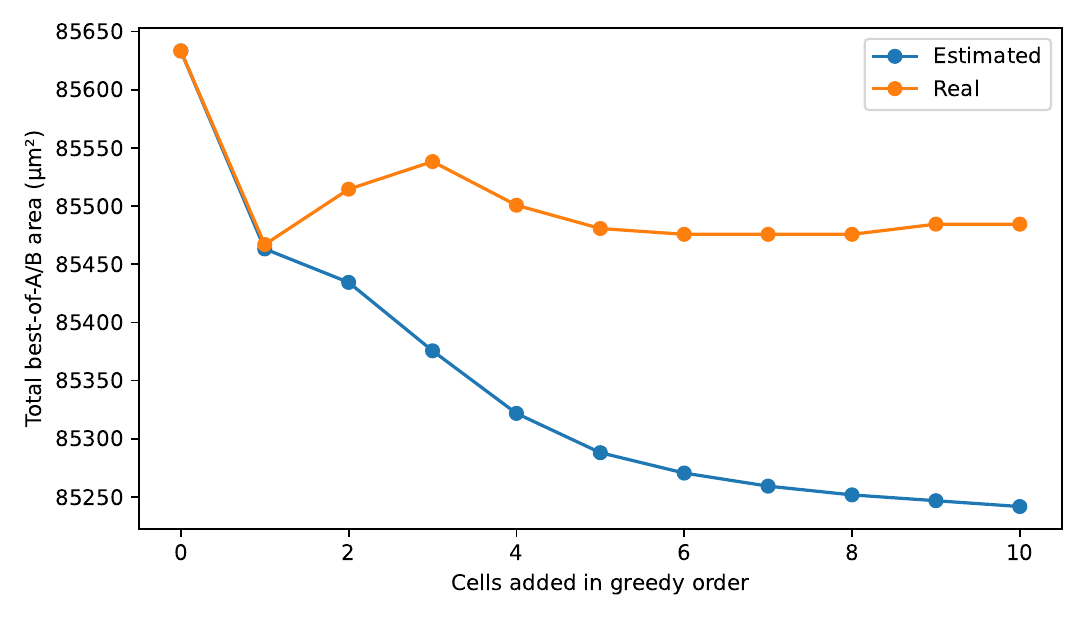
\includegraphics[width=0.8\linewidth]{m3/real/cell_curve.png}
    \caption{Total best-of-both area of the six required designs after each cell, in greedy order, with estimated and with real areas.}
    \label{fig:cell-curve}
\end{figure}

\begin{table}[h]
\centering\small
\caption{Curve values (\file{cell_curve_estimated.csv}, \file{cell_curve_real.csv}); total best-of-both area in \um.}
\label{tab:curve}
\setlength{\tabcolsep}{3.2pt}
\begin{tabular}{@{}lrrrrrrrrrrr@{}}
\toprule
Cells & 0 & 1 & 2 & 3 & 4 & 5 & 6 & 7 & 8 & 9 & 10 \\
added & -- & \cell{1bff} & \cell{00ae} & \cell{07ff} & \cell{ead5} & \cell{008a} & \cell{8aa0} & \cell{88f8} & \cell{aaae} & \cell{000e} & \cell{2e} \\
\midrule
Estimated & 85{,}633.4 & 85{,}463.2 & 85{,}434.4 & 85{,}375.6 & 85{,}321.8 & 85{,}288.0 & 85{,}270.5 & 85{,}259.3 & 85{,}251.8 & 85{,}246.8 & 85{,}241.8 \\
Real & 85{,}633.4 & 85{,}467.0 & 85{,}514.5 & 85{,}538.3 & 85{,}500.8 & 85{,}480.7 & 85{,}475.7 & 85{,}475.7 & 85{,}475.7 & 85{,}484.5 & 85{,}484.5 \\
\bottomrule
\end{tabular}
\end{table}

With estimated areas the curve falls monotonically, as the greedy rule guarantees: the first cell saves
170.2~\um, the last three together 17.5~\um{} (fewer than 12 of $\sim$770 trials improved in each of rounds
7--10). With real areas the curve is not monotonic and reaches its lowest point (85{,}467.0) after the first
cell; since no real cell is ever instantiated, the changes come from remapping alone (\S\ref{sec:area}).

\subsection{The 30\% experiment}
\label{sec:sens}

The first chosen cell, \cell{n4_1bff}, was made 30\% smaller (\file{sensitivity.json} in each run):

\begin{itemize}
\item \textbf{Estimated:} 13.76 $\to$ 9.63~\um. The six-design total fell from 85{,}241.8 to 85{,}144.3~\um,
so the saving rose from 0.457\% to 0.571\%. Script B then used \cell{n4_1bff} 143 times in risc8, 196 in pic16,
197 in p16c5x and 18 in cpu8, up from at most one instance per mapping.
\item \textbf{Real:} 75.07 $\to$ 52.55~\um. The cell is still never instantiated, yet the total \emph{rose}
from 85{,}484.5 to 85{,}518.3~\um{} (saving 0.174\% $\to$ 0.134\%), because risc8~B moved from 27{,}945.6 to
27{,}979.3~\um.
\end{itemize}

ABC sees only the Liberty numbers, so a small change in one area changes which cells \texttt{\&nf} uses by
the hundreds when the cell is competitive, and it moves the area by about 34~\um{} even when the cell stays
unused. The estimated result therefore depends strongly on the area estimate, and the real result is of the
same order as this library-induced variation.

%======================================================================
\section{Discussion}
\label{sec:disc}

\subsection{Classes}
We find 306 (synth) and 293 (restructured) four-input classes up to input order and output inversion in
the six required designs, and 73 and 81 NPN classes (Table~\ref{tab:aig}). The first count is the one
that matters for CMOS because a complementary stage gives the inverted output for free while each inverted
input needs a two-transistor inverter and adds a stage; two functions in one NPN class can therefore differ by
up to eight transistors and a stage. For all functions that depend on four inputs the same holds: the 3{,}904 P-classes form 1{,}952 PN
classes but only 208 NPN classes (computed with \file{dd2/boolfn.py}), and HD provides only 24 of the
3{,}904 (Table~\ref{tab:t4}).

\subsection{Redundancy}
Of the 833 candidate functions, the redundancy check dropped 55: 53 Exists (including every 2-input function)
and 2 Exists-with-an-inverter. Most of the HD-covered functions are the very frequent ones: \texttt{nand2},
\texttt{nor2}, \texttt{o21ai}, \texttt{xnor3}, \texttt{nand2b}/\texttt{and2b} and \texttt{xnor2} are 6 of the
8 most frequent mapped functions; the other two are 4-input parity functions. The Exists-with-an-inverter and Contained classes that survived were all
estimated smaller than the HD cell plus inverter, or than the containing HD cell. Two of the ten final cells
(\cell{n4_88f8}, \cell{n3_2e}) are Exists-with-an-inverter and one (\cell{n4_07ff}) is Contained in
\cell{a32oi_1}; with real areas none of these three beats the HD alternative (real 87.58, 30.03 and 16.27~\um{}
against 8.76+3.75, 10.01+3.75 and 8.76~\um).

\subsection{Area, and why the saving differs between designs}
\label{sec:area}

\textbf{Estimated cells.} Script~A used only cells whose expression uses every input once (\cell{07ff},
\cell{88f8}, \cell{00ae}, \cell{008a}, \cell{aaae}); \cell{n4_1bff}, in which A appears twice, appeared only under
script~B, in line with the handout's observation about \texttt{amap}. The best-of-both saving is largest on
fir10 (0.51\%, 36 instances of \cell{07ff}, $\overline{D(C+AB)}$, in script~A) and on
risc8 (0.72\%, where the script-B mapping becomes the better one). It is zero on cpu8 because script~A, which
gives its best area, uses no new cell. Same-script and best-of-both can disagree: fir10~B saves 0.99\% but
fir10's best area is script~A's; dsp8~B grows by 0.66\% while dsp8~A shrinks by 0.24\%. Three cells kept by
the greedy step (\cell{ead5}, \cell{8aa0}, \cell{n3_2e}) have no instance in any final mapping: their effect on the total was
through ABC's choices, not through their own use.

\textbf{Real cells.} The generator built every request, but its cells are 2.2--8.8$\times$ the estimate:
\cell{n4_88f8}, \cell{n4_ead5} and \cell{n4_8aa0} are 70--100 sites wide for 14--20 transistors, while the
4-input x1 cells of the reduced HD library are 5--10 sites wide. Even the most compact one, \cell{n4_07ff} (8 transistors in one
stage, like our estimate), takes 13 sites, where HD's \cell{a32oi_1} computes the same function in 7. ABC
therefore never used them (0 instances in 20 mappings). The 148.9~\um{} real saving is entirely risc8~B, a
remapping of existing HD gates by \texttt{\&nf} once the library changed; it is not attributable to the new
functions, and the 30\% experiment shows that such remapping moves the total by tens of \um{} by itself.

\textbf{Delay.} With estimated cells the new cells carry placeholder timing, so their delays only show that
nothing broke. With real cells the delay changes are again remapping effects: risc8~B improves from 25.65 to
18.37~ns and p16c5x~B from 27.51 to 21.79~ns, while fir10~B worsens from 7.64 to 8.38~ns (+9.7\%) and pic16~B
from 27.11 to 27.54~ns. On the required designs the only real best-of-both saving (risc8~B) is also faster; on the
held-out pic16, script~B saves 0.33\% with a 1.6\% longer worst arrival.

\textbf{risc8, pic16 and p16c5x.} The three implementations of the PIC16C5x instruction set favour the same
cells. With estimated areas, script~A uses exactly \{\cell{008a}, \cell{00ae}, \cell{07ff}\} on pic16 (3/5/4
instances) and on p16c5x (2/6/4), and \{\cell{00ae}, \cell{07ff}\} on risc8 (3/4); under script~B \cell{07ff} dominates
on all three (5, 25 and 20 instances). The two held-out designs saved 0.34\% and 0.21\% best-of-both, close to
risc8's 0.72\% and the 0.457\% of the objective. With real cells, risc8 and pic16 both improve through script~B
(0.53\% and 0.33\%) while p16c5x's best remains script~A and saves nothing.

\textbf{SPM.} In M2, SPM~B used 31 instances of \texttt{4:0xE888}, $(A{+}B)(AB{+}CD)$, and SPM's best-of-both
fell by 1.35\% (\file{results/m2/summary.md}). That cell was not selected in M3 because SPM is not in
the six-design objective and the cell did not help the required designs; in M3, SPM uses no new cell.

\subsection{Frequency against saving}
\label{sec:freq}

\textbf{A frequent function that cannot save area:} \texttt{4:0x9669}, four-input XNOR (parity). It is the
fifth most frequent function in our mapped cones (1{,}983 occurrences; 749 in the synth AIG cuts), it is New
(HD stops at \cell{xor3}/\cell{xnor3}), and it has no single-stage form. Our cheapest realization is a NAND network of 132
transistors in 11 stages, estimated at 65.06~\um, while the mapped designs implement it with XOR2/XNOR2 trees of about $3\times 8.76$~\um. No
occurrence's reclaimable area exceeds the cell's, so its predicted saving is 0 and adding it never changed the
total in any of the ten greedy rounds (\file{selection_trials.csv}).

\textbf{A frequent, cheap, ranked-first function that did not save:} \texttt{4:0x17FF},
$\overline{D\cdot\mathrm{maj}(A,B,C)}$, one stage with 12 transistors (8.76~\um), 231 mapped occurrences and
first in the ranking with a predicted 1{,}778~\um. Added alone it \emph{increased} the six-design total by
1.25~\um; in later rounds it never was the best candidate. B is the only script that uses a cell with a repeated
input, and B is not the better script for most of these designs, so the occurrences counted on the B netlists
did not reach the best-of-both total; the cut-based count also ignores that ABC restructures the logic around a
new cell. Frequency counts where a function \emph{could} go, not where ABC \emph{will} put it.

%======================================================================
\section{Limitations}
\label{sec:limits}

\begin{itemize}
\item \textbf{Area model.} The features come from our own explicit realizations, not from transistors
extracted from HD layouts, so they miss HD's custom layouts (XOR, small NAND/NOR) and diffusion sharing;
\cell{buf_1} is costed as a wire. The model has a 14.6\% leave-one-out error on HD and, more importantly, does
not describe the generator: its cells were 2.2--8.8$\times$ our estimates. Cells with more than four inputs are
excluded from the fit.
\item \textbf{Liberty file.} Estimated cells have a fixed input capacitance and scalar 0.10~ns placeholder
timing, so their OpenSTA delays are not meaningful; only the real cells carry characterized tables. One drive
strength (x1) is requested per function, while HD offers x2 and more.
\item \textbf{The two scripts.} \texttt{amap} (script~A) never used a cell with a repeated input, and
\texttt{\&nf} (script~B) is sensitive to any library change, including unused cells. Neither sees placement,
wiring or the larger pin access of a wider cell. Areas are cell areas only.
\item \textbf{Ranking and selection.} The ranking ignores overlap between candidates; the greedy search uses
the same six designs it reports, so the 0.457\% is an in-sample result (pic16 and p16c5x are the held-out check).
Selection was done with estimated areas, before real cells existed.
\item \textbf{Checks.} ABC \texttt{cec} proves combinational equivalence with aligned state; the Yosys
sequential induction is only a bounded diagnostic. Gate-level simulations are functional and zero-delay, and
cover only SPM and the multiplier. OpenSTA results are pre-layout comparisons under declared constraints.
\item \textbf{Tools.} Table~1 is reproduced with Yosys~0.33; M2 and M3 use Yosys~0.70+240, so their baseline
areas differ from Table~1. Within each run baseline and extended libraries use the same tool.
\end{itemize}

======================================================================
\section{Contributions}
\begin{itemize}
\item \textbf{Noor Elshahidi:} AIG extraction, cut enumeration and its checker, P/PN/NPN classes, and the redundancy checker with the Table 4 self-test.
\item \textbf{Mohamed Azouz:} Static-CMOS costing, the area model, mapped-cone ranking, the Appendix A requests and the Liberty writer.
\item \textbf{Omar Abdel Motalb:} A/B mapping with cec, OpenSTA and simulation, the greedy selection, the real generator cells and the 30\% experiment.
\end{itemize}

======================================================================
\appendix
\section{Tool versions}

\begin{table}
\centering\small
\begin{tabular}{@{}ll@{}}
\toprule
Tool & Version (from \file{results/m1/environment.json}, \file{results/m2/environment.json}) \\
\midrule
Yosys and bundled ABC (Table 1, M1) & Yosys 0.33 (git sha1 2584903a060) \\
Yosys and bundled ABC (M2, M3) & Yosys 0.70+240 (git sha1 5cdfd1241), OSS CAD Suite 2026-10-27 \\
Icarus Verilog & 14.0 (devel) (s20260301-739-gd95f2401b) \\
OpenSTA & 3.1.0 \\
Python & 3.12.3, with numpy 2.5.4 and matplotlib 3.11.2 (\file{results/m2/python_packages.txt}) \\
Cell generator & CellWeaver scl-gen 0.1.0 (\file{libs/cellweaver/responses.json}) \\
PDK & sky130A, \file{sky130_fd_sc_hd__tt_025C_1v80.lib} (SHA-256 \texttt{ec0e1067\ldots}) \\
Host & Ubuntu on WSL2 (Linux x86\_64) \\
\bottomrule
\end{tabular}
\end{table}

\end{document}